\begin{frame}
    \frametitle{What is Rust?}

    \begin{quote}{rust-lang.org}
    \centering
        A language empowering everyone\\
        to build reliable and efficient software.
    \end{quote}
\end{frame}

\begin{frame}
    \frametitle{Why Another Language?}

    \begin{itemize}
        \item We have plenty of languages to build reliably software:
        \begin{itemize}
            \item Java, C\#, Go, Python, Ruby, \dots
            \item All of these trade performance for safety
            \item All of them have a runtime (garbage collector, \dots)
        \end{itemize}

        \pause

        \item We have plenty of languages to build efficient software:
        \begin{itemize}
            \item C, C++, D, Assembly, \dots
            \item All of them trade safety for performance
        \end{itemize}

        \pause

        \item System programming requires efficiency/control \emph{and} safety!
    \end{itemize}
\end{frame}

\begin{frame}
    \frametitle{But Good Developers Don't Need Safety!}

    \pause

    \begin{tikzpicture}
        \draw (0, 0) node[inner sep=0] {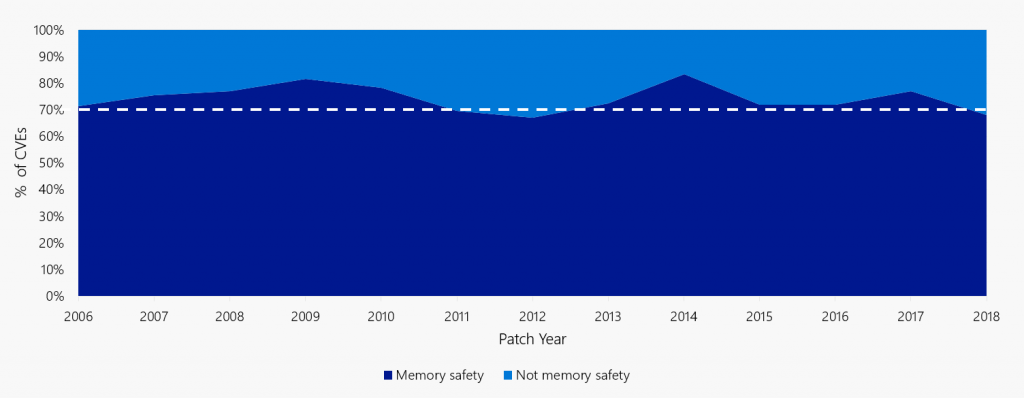
\includegraphics[width=\textwidth]{img/microsoft-memory-safety-trends.png}};
        \pause
        \draw (0, 0) node[fill=white,text=red,rotate=45] {\huge{We are using the wrong tools!}};
    \end{tikzpicture}
\end{frame}

\begin{frame}
    \frametitle{General Idea of Rust}

    \begin{itemize}
        \item C/C++ declare everything that is unsafe as ``undefined behavior''
        \begin{itemize}
            \item That pushes the problem to the developer
            \item There is no way out: the developer has the control all the time
        \end{itemize}

        \pause

        \item Rust provides safety without undefined behavior by default
        \begin{itemize}
            \item The developer can opt out by marking code as ``unsafe''
            \item The developer \emph{only} has the control if explicitly requested
        \end{itemize}

        \pause

        \item Rust tracks ownership at compile time and thereby is
        \begin{itemize}
            \item memory safe
            \item data-race free
        \end{itemize}
    \end{itemize}
\end{frame}

\begin{frame}
    \frametitle{Agenda}

    \begin{block}{Morning}
    \begin{itemize}
        \item Getting started
        \item Ownership
        \item Basic features + exercise
        \item Structs and enums + exercise
    \end{itemize}
    \end{block}

    \pause

    \begin{block}{Afternoon}
    \begin{itemize}
        \item Generics, traits, and error handling + exercise
        \item Unsafe, FFI, interior mutability
        \item Exercise: implement semaphores for a small kernel
    \end{itemize}
    \end{block}
\end{frame}

\begin{frame}[fragile]
    \frametitle{Repository}

    \Large
    To get the slides and the exercises:
    \begin{lstlisting}[language=bash,basicstyle=\large\ttfamily]
    $ git clone https://github.com/Nils-TUD/sysprog-rust.git
    \end{lstlisting}
\end{frame}
